\chapter{Luftbetankungstechnik}\label{cha:SdT}
Die Technologie der Luftbetankung ist seit 1917 ein gängiges Verfahren, welches in größerem Umfang im militärischen Bereich eingesetzt wird \cite{Methoden}. Durch die Herausforderung die Luftmobilität weiter auszubauen und gleichzeitig die umweltschädlichen Emissionen zu reduzieren unter der Bewältigung der Ziele des ACARE (Advisory Council for Aeronautics Research in Europe), versuchen Forscher weltweit diese Technologie auch auf zivile Anwendungen zu übertragen. Dabei sind folgenden Unterschiede zwischen der militärischen und zivilen Herangehensweise zu beachten \cite{CEAS2015}
\begin{itemize}
   
    \item Die Luftbetankung für ein Passagierflugzeug findet höher (ab 5 km) statt.
    \item Der zivile Tanker muss in der Lage sein, mehr als 4 Betankungsmissionen durchzuführen, ohne landen zu müssen, um den Vorgang wirtschaftlich rechtfertigen zu können.
\end{itemize}

Der Prozess moderner Luftbetankungsvorgänge verläuft wie folgt: Zuerst werden der Kraftstoffempfänger und der Kraftstoffspender verbunden. Nach erfolgreicher Verbindung wird das Kraftstoffsystem  automatisch mit dem Kraftstoffs Kreislauf verbunden. Nach Abschluss des Betankungsvorgangs wird die Empfangsmaschine gemäß dem Befehl der Betankungsmaschine getrennt und es wird somit der gesamte Betankungsprozess erfolgreich abgeschlossen.\\
Dabei ist die \textit{Probe-and-drogue} Methode das meist verwendete Betankungssystem \cite{Methoden}. Es bezieht sich auf einem flexiblen Ausleger, der den Tanker mit dem Passagierflugzeug verbindet. Der Ausleger selbst wird nicht gesteuert (passiv) und unterliegt externen aerodynamischen Einflüssen. Die Vorteile dieser Methode gegenüber anderer Varianten wie des \textit{Flying Boom} sind folgendermaßen aufgelistet \cite{Methoden}
\begin{itemize}
    \item Leicht und kompakt.
    \item Tanker kann mehrere Flieger oder Hubschrauber gleichzeitig bedienen.
    \item Einfache Anpassung für verschiedenen Geschwindigkeiten. 
\end{itemize}
Nachteilig ist die zusätzliche Belastung für den Piloten, die bei Einfluss des Windes und durch Turbulenzen steigt.\\ 
Zur Zeit wird es angestrebt unbemannte Tankermaschinen zu entwerfen, die den Betankungsprozess möglichst autonom erledigen \cite{Autonom1,Autonom2}. Dies würde nicht nur ein präziseres und sichereres Andocken darstellen, sondern würde auch in einer finanziell attraktiveren Lösung für die autonome Luftbetankung resultieren.\\
Unabhängig davon, ob der Tanker seinen Zweck autonom oder bemannt erfüllt, ist es notwendig eine Regelung auszulegen, die ein robustes Andocken ermöglicht. Dabei ist es von großer Bedeutung, dass sowohl der Tanker als auch das Passagierflugzeug den gleichen Kurs abfliegen und beide Maschinen bestimmte Bewegungen identisch durchführen. Dies wäre für die Piloten eine sehr herausfordernde Aufgabe. Daher wird es im Rahmen dieser Arbeit erforscht, wie ein Verkopplungsregler dabei unterstützen kann. 
\section*{ Verkopplungsregler}
Im Bereich der Regelung von MIMO Systemen (Multi Input Multi Output) ergeben sich zusätzliche Freiheitsgrade, die bei SISO (Single Input Single Output) Systemen nicht vorhanden sind. Der Verkopplungsregler nutzt diese Freiheitsgrade, um bestimmte Zustände zu koppeln. Dadurch versucht dieser lineare Regler, während des Abklingens der Eigenbewegung, diese Zustände so schnell wie möglich gleich zu setzen. Außerdem, verhalten sich die gekoppelten Größen bei Angaben von Führungsgrößen und äußeren Anregungen identisch. Dies ermöglicht, dass der Ausleger einen geringeren Bewegungsspielraum aufweist, was zu einem sicheren Andocken führt. Die erwünschte Toleranz für \textit{State of the Art} Regelungen beträgt für militärische Einsätze $2$ cm \cite{Autonom1}.  Im Rahmen dieses Projekts wird es zusätzlich eine Robustheitsanalyse durchgeführt, die untersucht, wie sich die beiden Flugzeuge bei einer Massenänderung und dem Windeinfluss verhalten unter Berücksichtigung der Verkopplung.\\
Außerdem versucht man den Regler so zu entwerfen, dass eine externe Vorgabe einiger Zustände noch möglich ist, wobei man für diese Analyse einen Geradeausflug vor der Betankung voraussetzt. Abgesehen von den Voraussetzungen der Regelungen (Kapitel \ref{cha:Anforderungen}), müssen folgenden Konditionen während des ganzen Betankungsverfahrens unbedingt eingehalten werden
\begin{itemize}
    \item Passagierflugzeug wird kollisionsfrei betankt.
    \item Abstand der Flugzeuge überschreitet nie die maximale Länge des Auslegers. 
    
\end{itemize}
\section{Passagierflugzeug-Tanker Konfiguration}
Bei der Überlegung welche Passagierflugzeug-Tanker Konfiguration sich am besten für den Kraftstoffaustausch eignet, werden folgenden Möglichkeiten in Betracht gezogen.
\begin{figure}[h]
\centering 
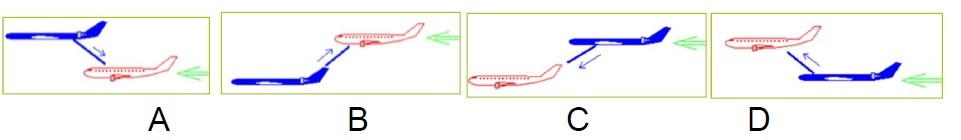
\includegraphics[scale=0.6]{./Bilder/Konfiguration.jpg}
\label{fig:Konfigurationen}
\caption{Bild der unterschiedlichen Flug Konfigurationen \cite{RefuelingTime}. Das blaue Flugzeug stellt den Tanker und das rote das Passagierflugzeug dar.}
\end{figure}

Dabei wählt man für dieses Projekt die Option D, da folgenden Vorteile erzielt werden \cite{RefuelingTime}
\begin{itemize}
    \item Kein Kolisionsrisiko für das Passagierflugzeug aufgrund ablösender Teile des Tankers.
    \item Der Pilot des Passagierflugzeugs muss keine Annährungsmanöver fliegen.
    \item Passagiere unterliegen keiner Manöverbeschleunigung, was zu einem höheren Komfort führt.
    \item Nur der Tanker muss mit einem \textit{Air to Air} Radar ausgerüstet sein.
    \item Zustände des Passagierflugzeugs werden weniger von der Anwesenheit des Tankers beeinflusst.
\end{itemize}
Nachteilig ist der zusätzliche Bedarf einen nach vorne ausgerichteten Ausleger anzuwenden, welcher anfälliger bezüglich Störungen ist. Dies wäre ein zusätzliches Argument einen robusten Verkopplungsregler einzusetzen, der trotz Störungen eine sichere Betankung ermöglicht.
